\begin{figure}[H]
\begin{lstlisting}[
language={[x86masm]Assembler},
caption={Assembly Code for AND Subroutine},
label=ANDRoutine
]
JUN START
AND FIM 1 0 11
Loop LDM 0
XCH 0
RAL
XCH 0
INC 3
XCH 3
JCN 4 Done
XCH 3
RAR
XCH 2
XCH 1
RAL
XCH 1
RAR
ADD 2
JUN Loop
Done BBL 0
START LDM 11
XCH 0
LDM 6
XCH 1
JMS AND
NOP
\end{lstlisting}
\end{figure}

The AND subroutine produces the AND of two input words by placing the bits in the leftmost position of the accumulator \ref{ACC} and register 2 \ref{Scratch2}, respectively, and zeroing the rightmost three bits of the accumulator and register 2. Register 2 is then added to the accumulator, and the resulting carry is equal to the AND of the two bits. Scratch Pad register 3 (Figure \ref{Scratch3}) is used as the counter, counting up from 11. When this overflows from 15 to 0 the program breaks and returns.

\begin{figure*}[h]
\centering
\subcaptionbox{Scratchpad 0 value, containing the first input word which is shifted left four times. This is the register the function returns the output value to. The shifts are as follows, 1011 to 0110 to 1100 to 1000. The returned value is then placed in and shifted once, 0001 to 0010.\label{Scratch0}}
{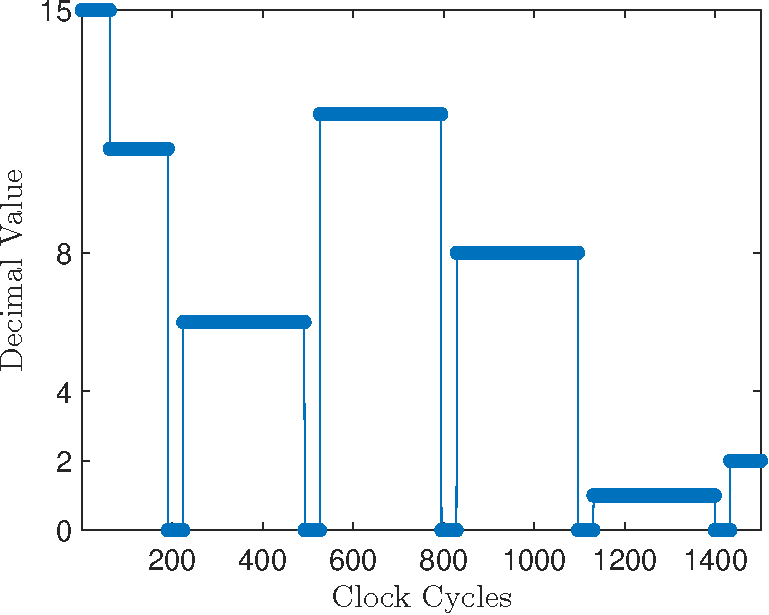
\includegraphics[width=0.49\linewidth, height = 0.2\textheight]{Appendices/Scratchpad0.pdf}}
\subcaptionbox{Scratchpad 1 value, containing the second input word which is shifted left three times. The shifts are as follows, 0110 to 1100 to 1000 to 0000.\label{Scratch1}}
{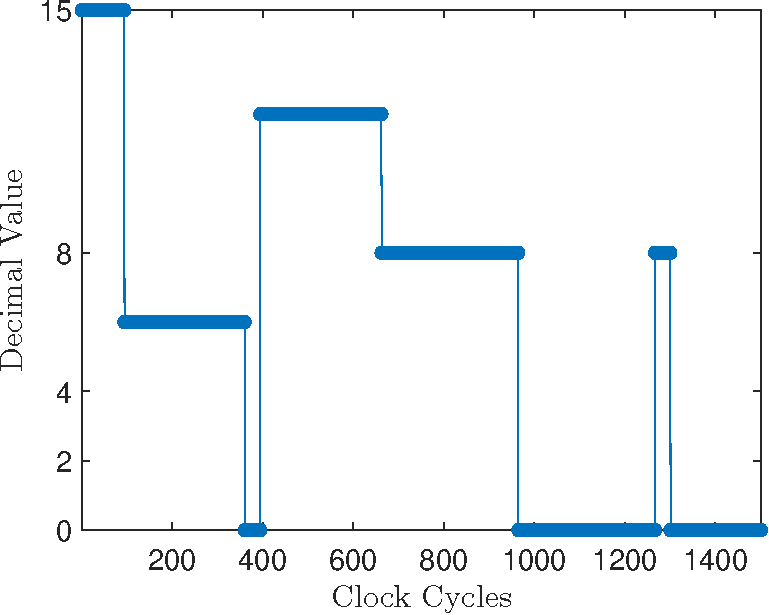
\includegraphics[width=0.49\linewidth, height = 0.2\textheight]{Appendices/Scratchpad1.pdf}}
\caption{Scratchpad Pair 0, the input and output registers.\label{Scratch00}}
\end{figure*}

\begin{figure*}[h]
\centering
\subcaptionbox{Scratchpad 2 value, this is working memory for the program. The highest order bit from one input is put into here and added to the accumulator which contains the high order bit from the other input.\label{Scratch2}}
{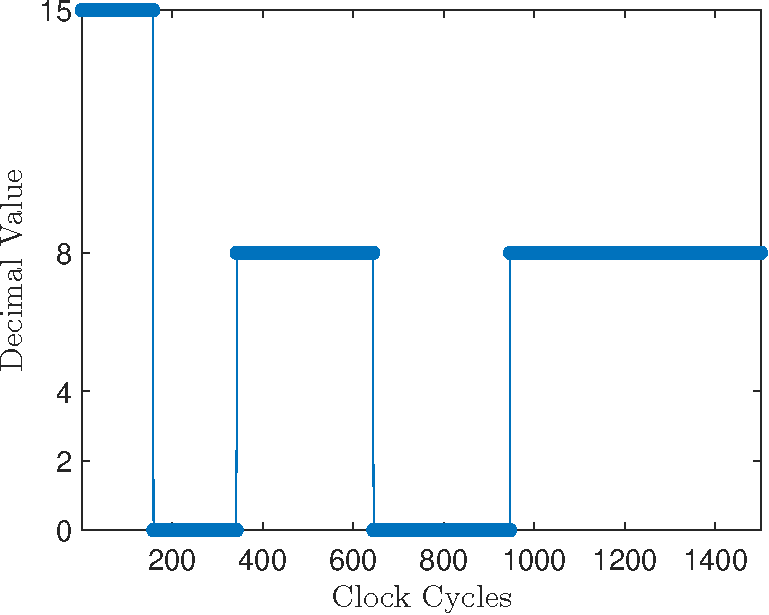
\includegraphics[width=0.49\linewidth, height = 0.2\textheight]{Appendices/Scratchpad2.pdf}}
\subcaptionbox{Scratchpad 3 value, this is the counter for counting the number of times register 0 has been shifted. This starts at 11 and the program breaks when the value overflows from 15 to 0.\label{Scratch3}}
{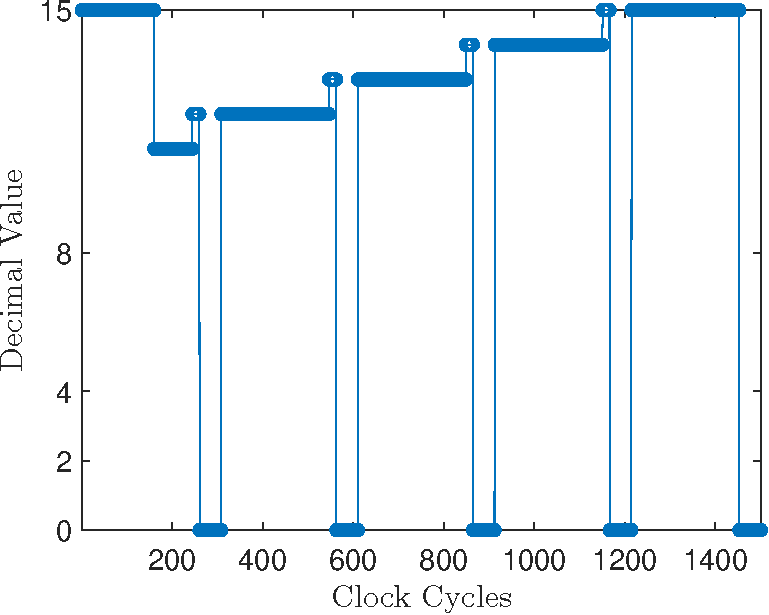
\includegraphics[width=0.49\linewidth, height = 0.2\textheight]{Appendices/Scratchpad3.pdf}}
\caption{Scratchpad Pair 1\label{Scratch01}}
\end{figure*}

\begin{figure*}[h]
\centering
\subcaptionbox{Accumulator register value\label{ACC}}
{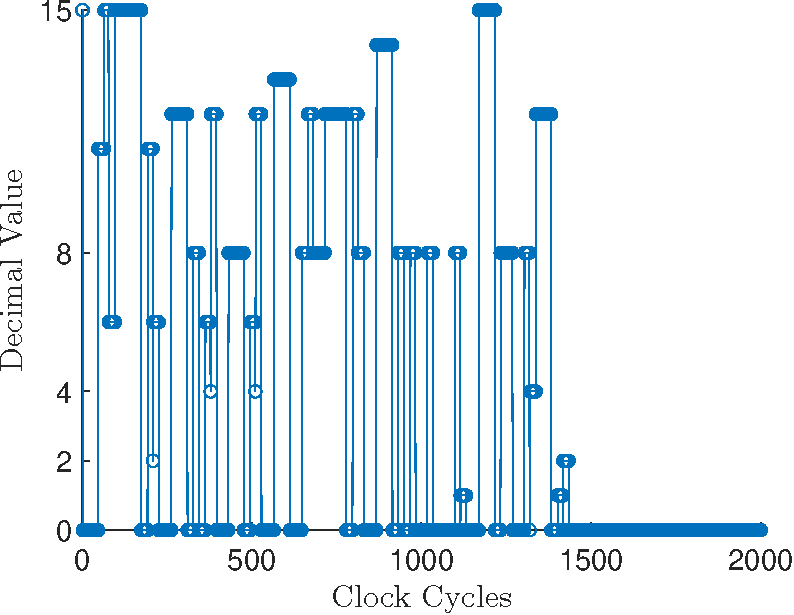
\includegraphics[width=0.49\linewidth, height = 0.2\textheight]{Appendices/ACC.pdf}}
\subcaptionbox{Carry Flag register value, when the highest bit of word one and word two are added together the carry is equal to the AND of the two bits\label{CF}}
{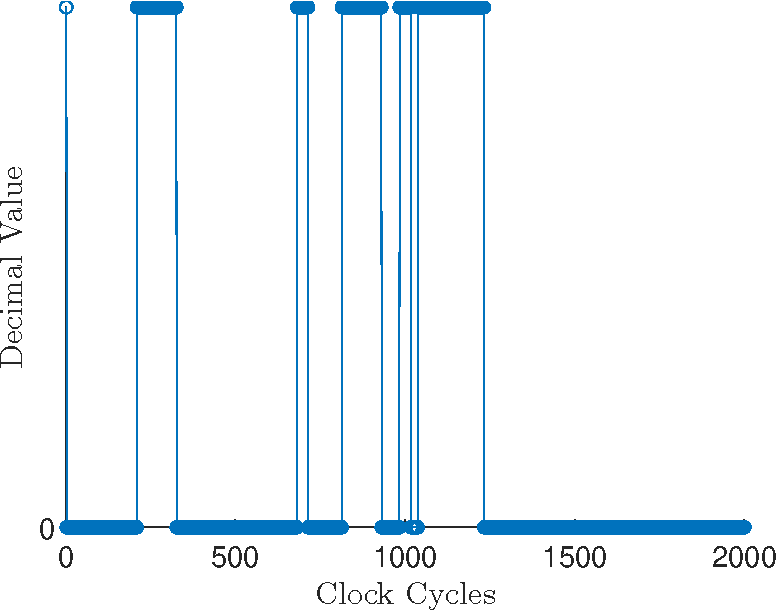
\includegraphics[width=0.49\linewidth, height = 0.2\textheight]{Appendices/CF.pdf}}
\caption{Accumulator and Carry Flag register values\label{ACCCF}}
\end{figure*}
